\documentclass[titlepage,a4paper,12pt]{article}

\usepackage[english,serbian]{babel}
\usepackage{mathptmx}
\usepackage{microtype}
\usepackage{graphicx}
\usepackage{wrapfig}
\usepackage{enumitem}
\usepackage{amsmath}
\usepackage{amsfonts}
\usepackage{listings}
\usepackage{xcolor}
\usepackage{placeins}
\usepackage{flafter}
\usepackage{enumitem}
\usepackage[normalem]{ulem}
\useunder{\uline}{\ulined}{}

\definecolor{codegreen}{rgb}{0,0.6,0}
\definecolor{codegray}{rgb}{0.5,0.5,0.5}
\definecolor{codepurple}{rgb}{0.58,0,0.82}
\definecolor{backcolour}{rgb}{0.95,0.95,0.92}

\lstdefinestyle{mystyle}{
	backgroundcolor=\color{backcolour},   
	commentstyle=\color{codegreen},
	keywordstyle=\color{magenta},
	numberstyle=\tiny\color{codegray},
	stringstyle=\color{codepurple},
	basicstyle=\ttfamily\footnotesize,
	breakatwhitespace=false,         
	breaklines=true,                 
	captionpos=b,                    
	keepspaces=true,                 
	numbers=left,                    
	numbersep=5pt,                  
	showspaces=false,                
	showstringspaces=false,
	showtabs=false,                  
	tabsize=2
}

\lstset{style=mystyle}

\renewcommand{\lstlistingname}{Kod}
\renewcommand{\lstlistlistingname}{Lista \lstlistingname ova}

\usepackage{tikz}
\usetikzlibrary{math}

\begin{document}	
	\tikzmath{
		integer \godina;
		\godina = 2020;
		integer \indeks;
		\indeks = 260;
		integer \varsum;
		\varsum = \indeks + \godina;
		integer \digsumindeks;
		\digsumindeks = \indeks / 1000 + Mod(\indeks / 100,10) + Mod(\indeks/10,10) + Mod(\indeks,10);
		integer \digsumgodina;
		\digsumgodina = \godina / 1000 + Mod(\godina / 100,10) + Mod(\godina/10,10) + Mod(\godina,10);
		integer \digsum;
		\digsum = \digsumindeks + \digsumgodina;
		integer \Nval;
		\Nval = Mod(\varsum,6);
		integer \Pval;
		\Pval = Mod(\varsum, 5);
		integer \Qval;
		\Qval = Mod(\digsum,5);
		integer \Rval;
		\Rval = Mod(\digsum,3);
	}
	
	\begin{titlepage}
		\begin{center}
			\vspace*{1cm}
			
			\Huge
			\textbf{Signali i sistemi}\\
			\LARGE
			\textbf{Domaci 1}
			
			\vspace{1cm}
			\Large
			
			Branislav Đumić\\
			Br. indeksa: 0\indeks/\godina
			\vfill
			
%			\begin{figure*}[ht]
%				\centering
%				\includegraphics[width=\textwidth]{Images/indeks.png}
%			\end{figure*}
			\vfill
			Parametri
			
			\vspace{0.25cm}
			\large
			N = \Nval, P = \Pval, Q = \Qval, R = \Rval
			
		\end{center}
	\end{titlepage}
	\normalfont
	\renewcommand{\contentsname}{Sadžaj}
	\tableofcontents
	\clearpage
	
	
	\section{Zadatak 1.}
	\Large{Osnovne osobine i vremenske transformacije signala}
	
	\subsection[Prvi deo]{Odrediti analitički izraz za signal $f(t)$ i nacrtati
		grafike signala $x(t)$ i $f(t)$.}
	\vspace{-15pt}
	\normalsize{}
	\begin{equation}
		f(t) = x(3(Q+3) - (R+1) t) \label{eq:zadatak11}
	\end{equation}
	\indent Zamenom parametara zadatka u izraz \eqref{eq:zadatak11} 	dobija se
	relacija koja povezuje signale $f(t)$ i $x(t)$.
	\begin{equation}
		f(t) = x(15 - t)
	\end{equation}
	\vspace{-0.1cm}
	\noindent Na ovoj slici može se videti postupak transformacije signala $x(t)$ u $f(t)$
	\begin{figure*}[ht]
		\centering
		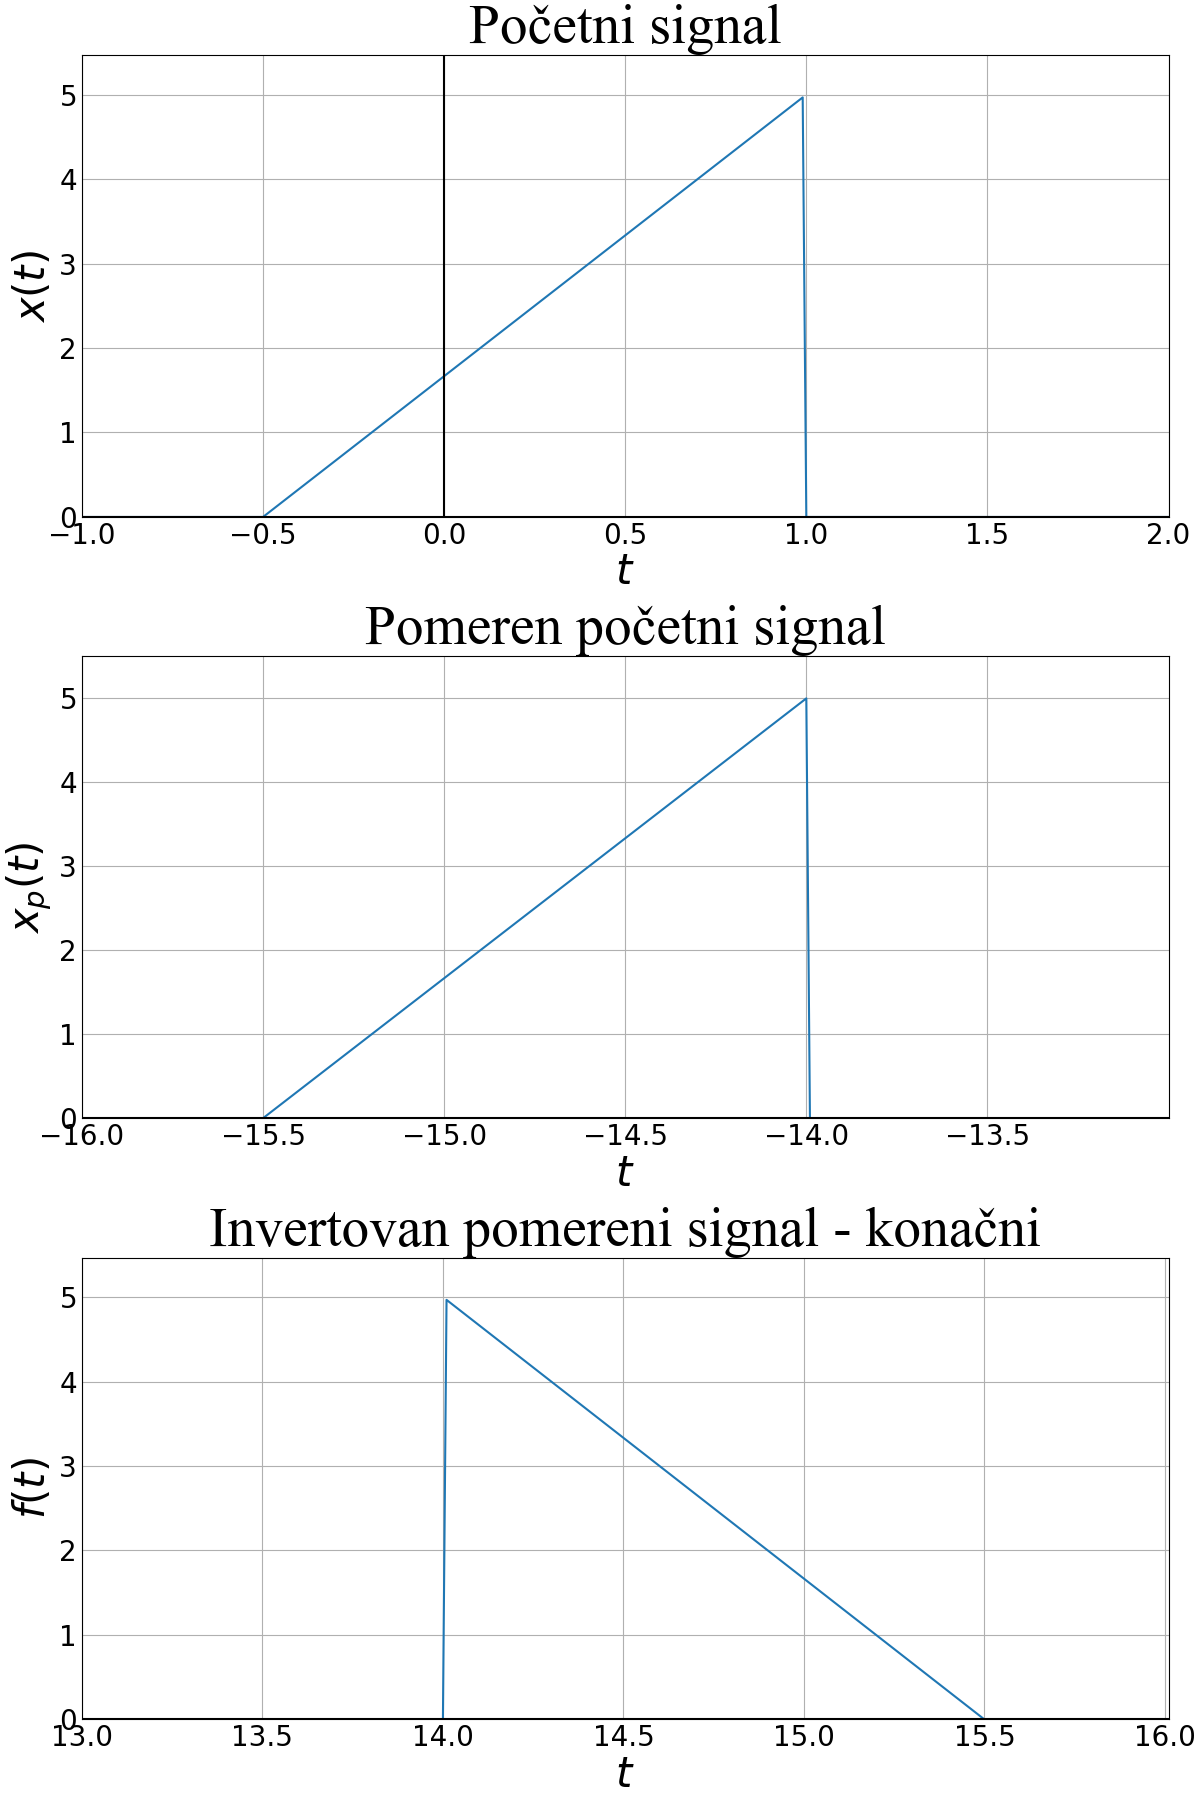
\includegraphics[width=8cm]{Images/zadatak1pic1.png}
		\caption{Transformacije $x(t)$ u $f(t)$}\label{fig:slika1}
	\end{figure*}
	\FloatBarrier
	\clearpage
	\indent Za skiciranje grafika koristi se sledeći kod u programskom jezuku
	Python:
	\lstinputlisting[language=Python, caption={Kod za generisanje grafika sa Slike
		\ref{fig:slika1}}]{Codes/zadatak1a.py}
	\vspace{10pt}
	\textbf{Orderđivanje analitičkog oblika}\label{findanalityc1}\\\\
	\normalsize{}
	\indent Sa slike se vidi da je signal $f(t)$ oblika:
	\begin{equation}
		f(t) = (at + b)\big( u(t-14) - u(t-15.5)\big) \label{eq:signalft}
	\end{equation}
	Zamenom poznatih parova tačaka $(t,f(t))$, $ A=(14,5)$ i $B=(15.5,0)$ u
	\eqref{eq:signalft} dobijamo :
	\begin{flalign}
		&f(14) = 14a + b = 5 \label{eq:findval1}\\
		&f(15.5) = 15.5a + b = 0 \label{eq:findval2}
	\end{flalign}
	\noindent{Oduzimanjem jednačina \eqref{eq:findval1} i \eqref{eq:findval2},
		dobija se $a=-\frac{10}{3}$ i $b=\frac{155}{3}$, tako da je konačan izraz za
		$f(t):$}
	\begin{equation}
		f(t) = \frac{5}{3}\big(-2t + 31\big)\big(u(t-14)-u(t-15.5)\big)
	\end{equation}

	\clearpage
	\subsection[Drugi deo]{Predložiti metodu interpolacije, pa na osnovu nje
		prikazati grafik i napisati analitički oblik signala:}
	\vspace{-15pt}
	\begin{flalign}
		v[n] = 2\cdot w\Big[\frac{n}{3}-2\Big]
	\end{flalign}
	\indent Na osnovu parametara zadatka dobija se da je oblik signala $w[n]$:
	\begin{equation}
		w[n] = 0.5^n\Big(u[n+2]-u[n-2]\Big)
	\end{equation}
	\indent Predlaže se metoda linearne interpolacije. Na ovoj slici može se videti
	postupak translacije signala $w[n]$ u signal $w[n-2]$. Uvode se novi signali
	$w_p[n]=w[n-2]$ i $r[n] = 2w_p[n]$. Konačan signal dobijamo skapiranjem i
	inerpolacijom signala iz $r[n]$, odnosno $v[n] = r[\frac{n}3]$
	\begin{figure*}[ht]
		\centering
		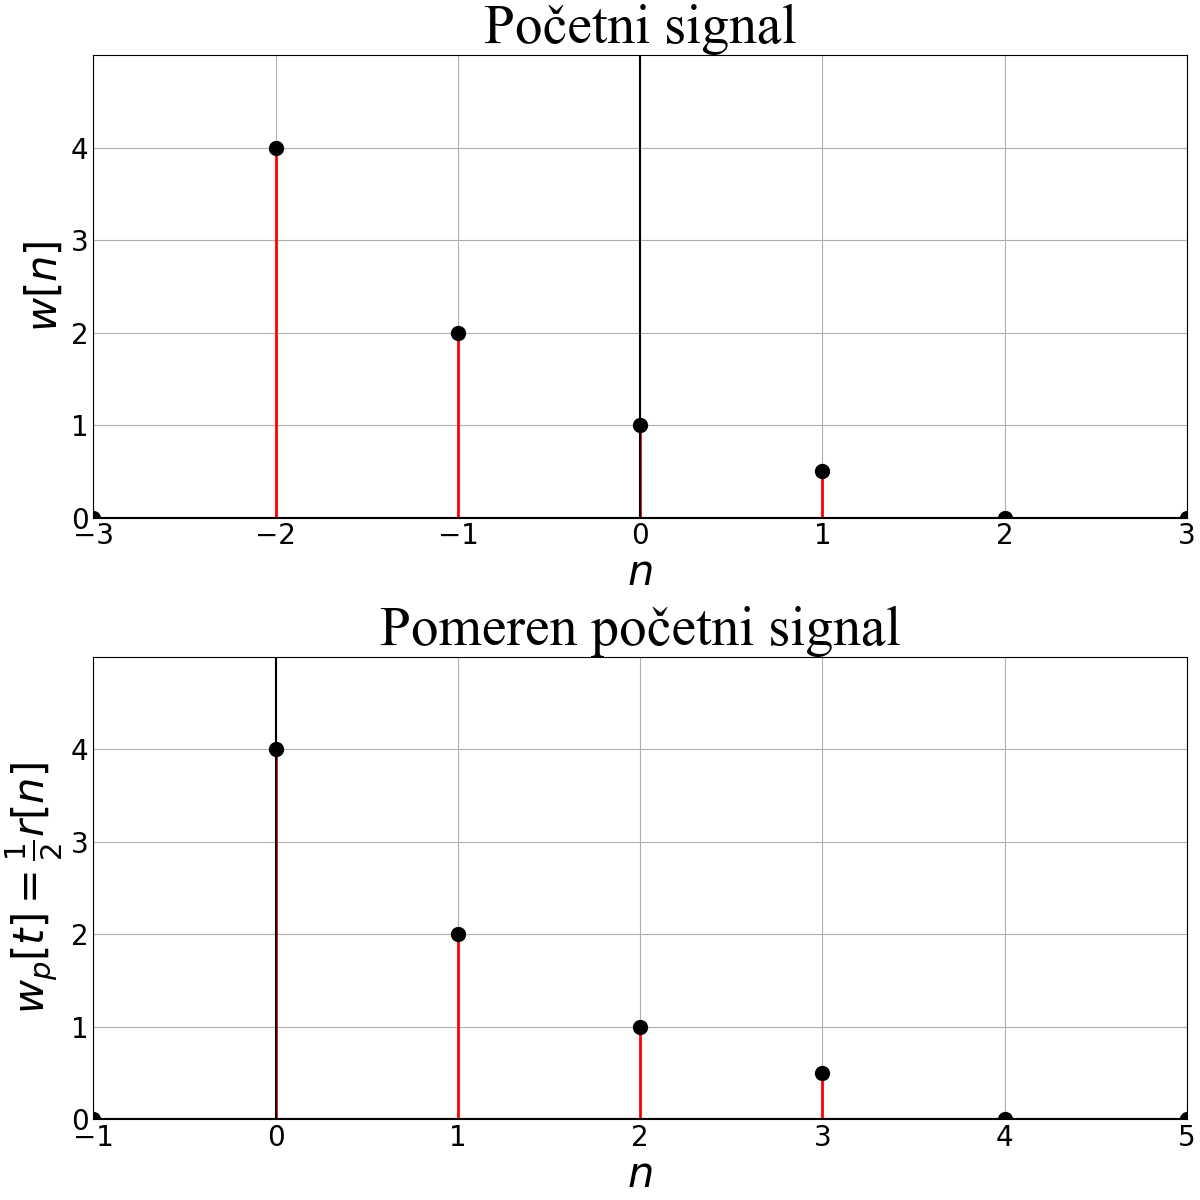
\includegraphics[width=10cm]{Images/zadatak1pic2.png}
		\caption{Transformacija $w[n]$ u $w[n-2]$}\label{fig:slika2}
	\end{figure*}
	\FloatBarrier
	\pagebreak
	\indent{Za skiciranje grafika korišćen je sledeći kod u programskom jeziku
		Python:}
	\lstinputlisting[language=Python, caption={Kod za generisanje grafika sa Slike
		\ref{fig:slika2}}]{Codes/zadatak1b.py}
	\indent{Nakon skapiranja, uz linearnu interpolaciju, rezultujući oblik signala
		$v[n]$ je:}
	\begin{equation}
		v[n] = \left\{
		\begin{array}{ll}
			r[k]&,\quad n = 3k \\\\
			\frac{2\cdot r[k]+r[k+1]}{3}&,\quad n = 3k + 1\\\\
			\frac{r[k]+2\cdot r[k+1]}{3}&,\quad n = 3k + 2 \\
		\end{array}\right.\label{eq:zadatak1bfinal}
	\end{equation}
	\indent{Kako bi skicirali konačan grafik(signal $g[n]$), potrebno je na osnovu
		izraza \eqref{eq:zadatak1bfinal} izračunati vrednosti signala $g[n]$. Vidimo da
		će vrednost signala biti nula za $n \le -3$ i $n \ge 12$, dok ostale vrednosti
		dobijamo direktnom zamenom.}
	\begin{flalign*}
		&v[-3] = r[-1] = 0 &&v[-2] = \frac{2\cdot r[-1] + r[0]}3 = \frac{4}{3} && v[-1] = \frac{r[-1] + 2\cdot r[0]}3 = \frac{8}{3}\\
		&v[0]=r[0]=8 && v[1] = \frac{2\cdot r[0] + r[1]}3 = \frac{20}{3} && v[2] = \frac{r[0] + 2\cdot r[1]}{3} = \frac{16}3 \\
		& v[3] = r[1] = 4 && v[4] = \frac{2\cdot r[1] + r[2]}3 = \frac{10}3 && v[5] = \frac{r[1]  + 2\cdot r[2]}3 = \frac{8}3 \\
		& v[6] = r[2] = 2 && v[7] = \frac{2\cdot r[2] + r[3]}3 = \frac{5}3 && v[8] = \frac{r[2]+2\cdot r[3]}3 = \frac{4}3 \\
		& v[9] = r[3] = 1 && v[10] = \frac{2\cdot r[3] + r[4]}3 = \frac{2}3 && v[11] = \frac{r[3] + 2\cdot r[4]}3 = \frac{1}3\\
	\end{flalign*}
	\clearpage
	\indent Kada unesemo ove vrednosti u grafik, dobijemo sledeću sliku:
	\begin{figure*}[ht]
		\centering
		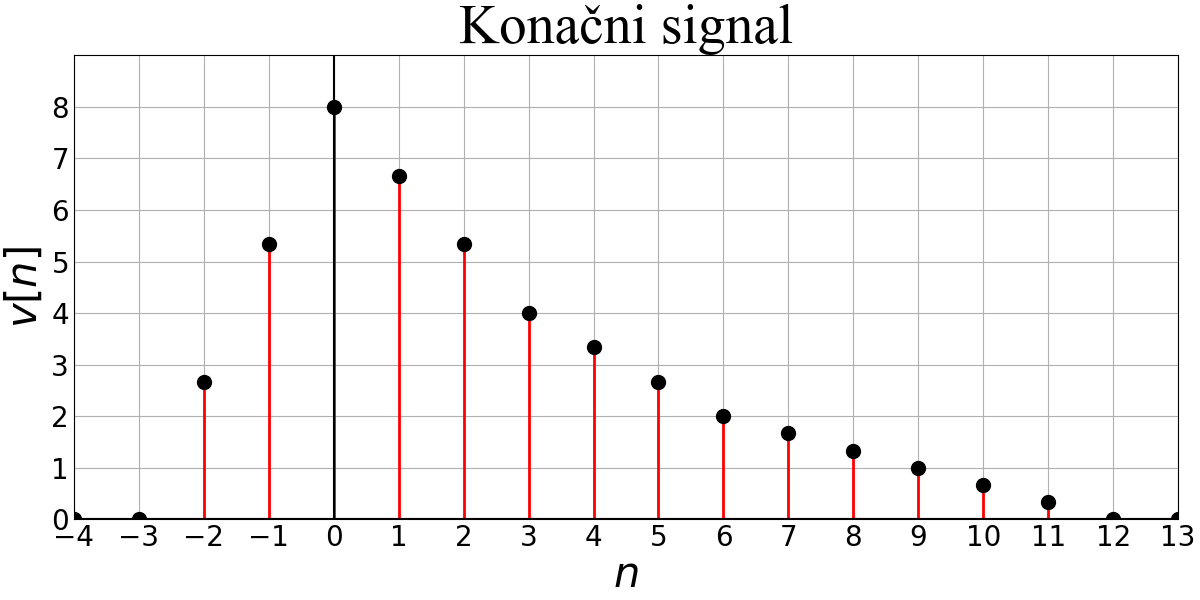
\includegraphics[width=11cm]{Images/zadatak1pic3.png}
		\caption{Konačan oblik signala $v[n] = 2w[\frac{n}3-2]$}\label{fig:slika3}
	\end{figure*}
	\FloatBarrier
	\indent{Za skiciranje grafika korišćen je sledeći kod u programskom jeziku
		Python:}
	\lstinputlisting[language=Python,caption={Kod za generisanje grafika sa Slike
		\ref{fig:slika3}.}]{Codes/zadatak1b2.py}
	
	\subsection[Treći deo]{Definisati paran i neparan deo signala $w[n]$. Prikazati
		grafike $w[n]$,  $E_v\{w[n]\}$,  $O_d\{w[n]\} $:}
	\indent Potrebno je odrediti vezu između signala $Ev\{w[n]\}$ i  $Od\{w[n]\}$
	sa signalom $w[n]$. Znamo da se svaki signal može predstaviti kao zbir parnog i
	neparnog signala, tako da imamo:
	\begin{equation}
		w[n] = Ev\{w[n]\} + Od\{w[n]\}\label{eq:evenoddrel}
	\end{equation}
	Ako zamenimo $n = -n$ u jednačinu \eqref{eq:evenoddrel} dobijamo:
	\begin{equation}
		w[-n] = Ev\{w[n]\} - Od\{w[n]\}\label{eq:evenoddrelmin}
	\end{equation}
	\noindent Kombinovanjem jednačina \eqref{eq:evenoddrel} i
	\eqref{eq:evenoddrelmin}
	\begin{flalign}
		w[n] + w[-n] = 2\cdot Ev\{w[n]\}
		\label{eq:evenoddsum}\tag*{\eqref{eq:evenoddrel} + \eqref{eq:evenoddrelmin}}\\
		w[n] - w[-n] = 2\cdot Od\{w[n]\}
		\label{eq:evenodddiff}\tag*{\eqref{eq:evenoddrel} - \eqref{eq:evenoddrelmin}}
	\end{flalign}
	\clearpage
	\noindent Iz ovih jednačina dobijaju se konačni oblici za signale $Ev\{w[n]\}$ i $Od\{w[n]\}: $
	\indent\begin{minipage}{0.5\textwidth}
		\begin{flalign}
			Ev\{w[n]\} = \frac{w[n] + w[-n]}{2}
		\end{flalign} 
	\end{minipage}%
	\begin{minipage}{0.5\textwidth}
		\begin{flalign}
				Od\{w[n]\} = \frac{w[n] - w[-n]}{2}
		\end{flalign}
	\end{minipage}\vskip1em
	\noindent Na sledećoj slici mogu se videti grafici signala $w[n]$, 
	$E_v\{w[n]\}$,  $O_d\{w[n]\}: $
	\begin{figure*}[ht]
		\centering
		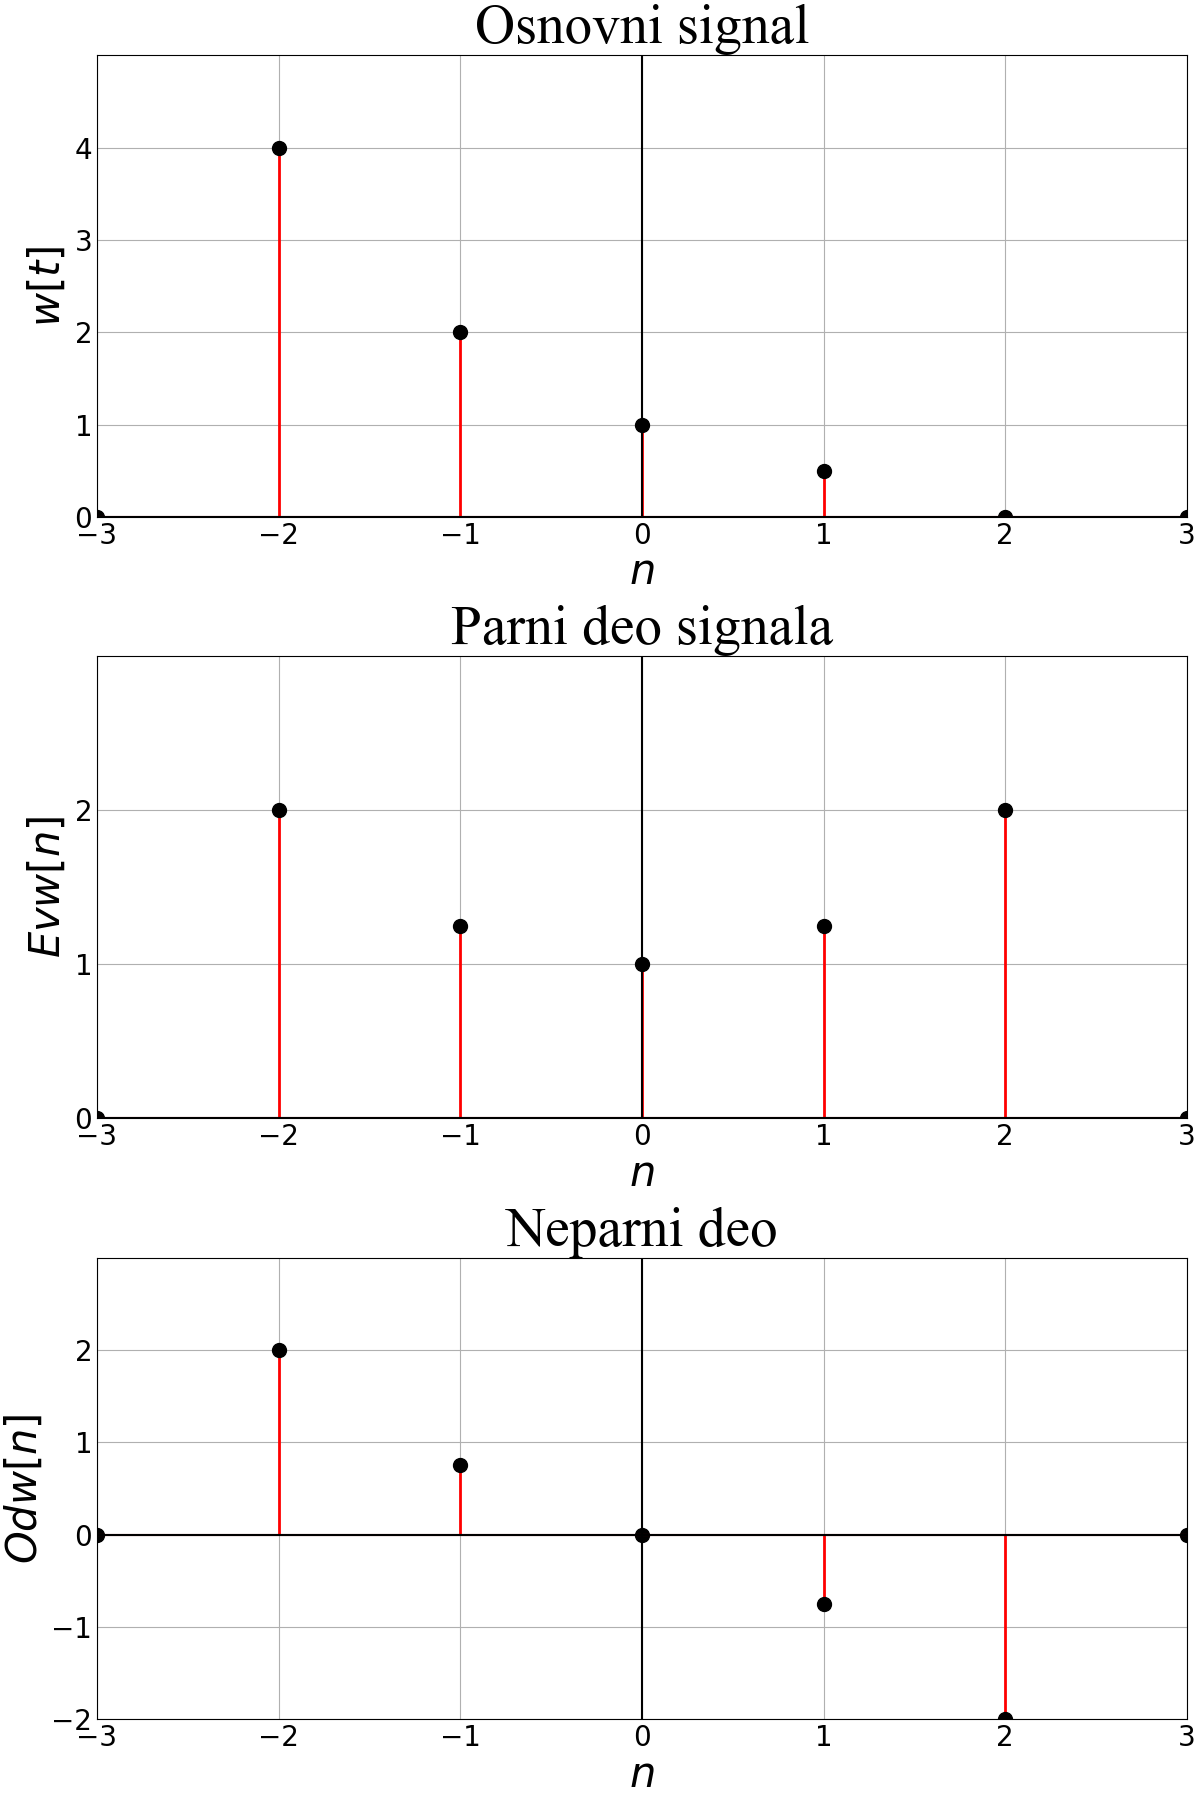
\includegraphics[width=10cm]{Images/zadatak1pic4.png}
		\caption{Signali $w[n]$, $Ev\{w[n]\}$ i $Od\{w[n]\}$}\label{fig:slika4}
	\end{figure*}
	\FloatBarrier
	\pagebreak
	\indent{Za skiciranje grafika korišćen je sledeći kod u programskom jeziku
		Python:}
	\lstinputlisting[language=Python,caption={Kod za generisanje grafika sa Slike \ref{fig:slika4}.}]{Codes/zadatak1c.py}
	\clearpage
	
	
	\section{Zadatak 2.}
	\Large{Konvolucija}
	\normalsize{}
	
	\subsection[Prvi deo]{Analitički odrediti i skicirati konvoluciju signala $x(t)$ i $y(t)$}
	\begin{figure*}[ht]
		\centering
		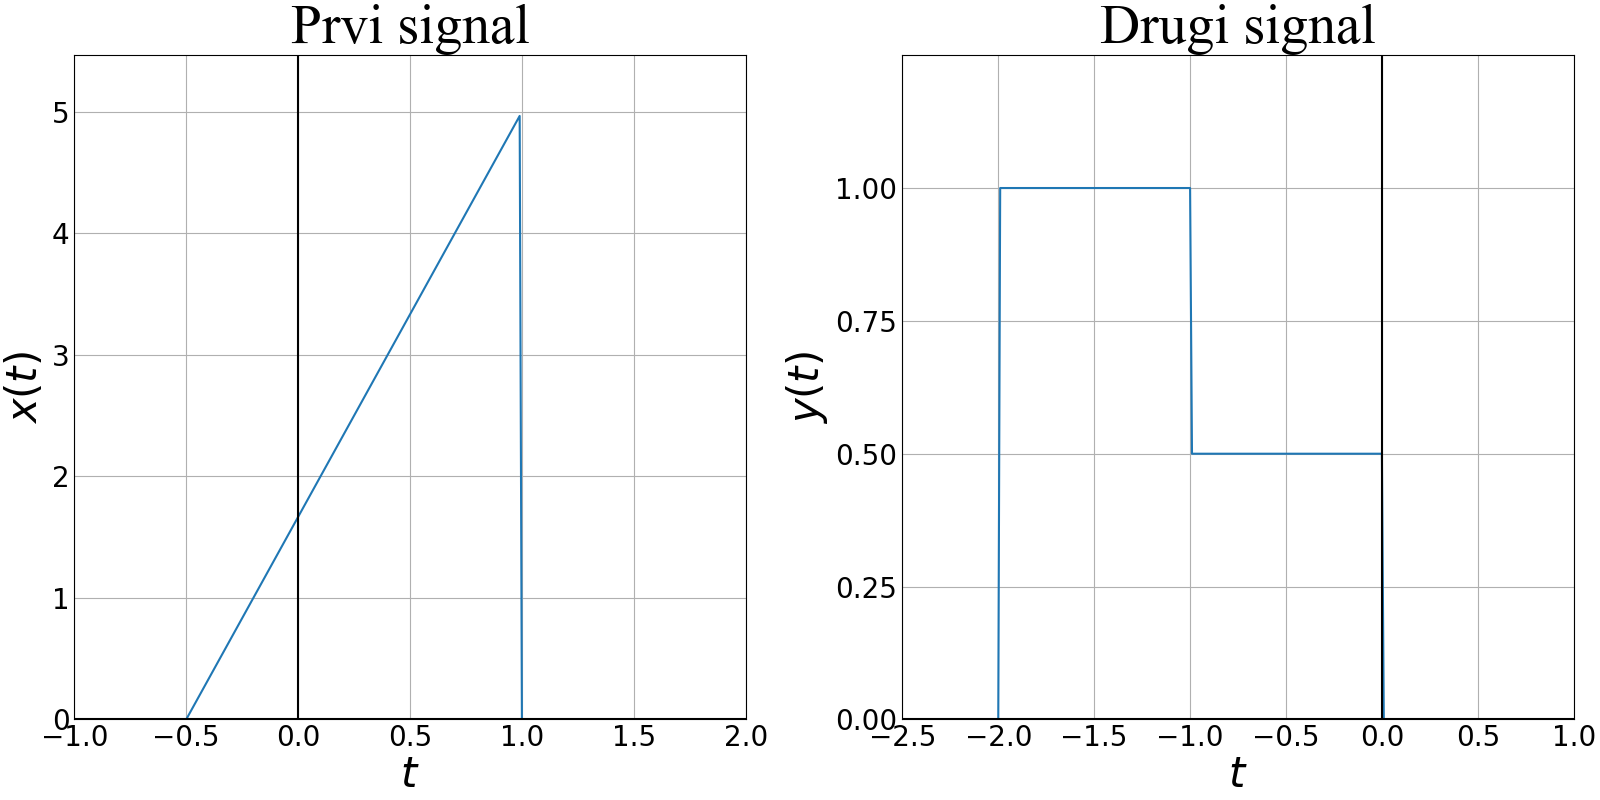
\includegraphics[width=\textwidth]{Images/zadatak2pic1.png}
		\caption{Signali $x(t)$ i $y(t)$}\label{fig:slika5}
	\end{figure*}
	\indent{Za skiciranje grafika korišćen je sledeći kod u programskom jeziku
		Python:}
	\lstinputlisting[language=Python,caption={Kod za generisanje grafika sa Slike \ref{fig:slika5}.}]{Codes/zadatak2a1.py}
	\clearpage
	\indent Postupkom kao u zadadtku \ref{findanalityc1} možemo odrediti analitički oblik signala $x(t)$, dok je oblik signala $y(t)$ jednostavno očitati sa slike. Primenom ovog postupka dobijamo:
	\begin{flalign}
		&x(t) = \frac{5}{3}(2t + 1)\big(u(t+0.5) - u(t-1)\big)\label{eq:xoftanalytic}\\
		&y(t) = u(t+2) - 0.5u(t+1) - 0.5u(t) \label{eq:yoftanalytic}
	\end{flalign}
	\indent Radi lakšeg nalaženja konvolucije signala $x(t)$ i $y(t)$, $z(t)=x(t)*y(t)$, razdvojićemo signal $y(t)$ na signale $y_1(t) = u(t+2) - u(t+1)$ i $y_2(t) = \frac{1}{2}\big(u(t+1) - u(t)\big)$, tako da je $y(t) = y_1(t) + y_2(t)$. Konvolucija je komutativna operacija, pa se konvolucija signala $x(t)$ i $y(t)$, nazovimo je $z(t)$, može definisati se kao:
	\begin{equation}
		z(t) = y(t) * t(t) = \int_{-\infty}^{+\infty}y(\tau)\cdot x(t-\tau)d\tau\label{eq:convolution}
	\end{equation}
	\indent Zamenom \eqref{eq:xoftanalytic} i \eqref{eq:yoftanalytic} u \eqref{eq:convolution} dobijamo:
	\begin{flalign}
		z(t) &\quad= \int_{-\infty}^{+\infty}\big(y_1(\tau) + y_2(\tau)\big) \cdot x(t-\tau)d\tau\notag\\	
		&\quad= \int_{-\infty}^{+\infty}y_1(\tau)\cdot x(t-\tau)d\tau + \int_{-\infty}^{+\infty}y_2(\tau)\cdot x(t-\tau)d\tau\notag \\
		z(t) &\quad= x(t) * y_1(t) + x(t) * y_2(t) \label{eq:sepconv}
	\end{flalign}
	\indent Neka je $z_1(t) = x(t) * y_1(t)$ i $z_2(t) = x(t) * y_2(t)$. Zbog distributivnosti operacije konvolucije u odnosu na operaciju sabiranja znamo da je $z(t) = z_1(t) + z_2(t)$. Prvo računamo signal $z_1(t)$:
	\begin{flalign*}
		z_1(t) &\quad= \int_{-\infty}^{+\infty}\Big[u(\tau+2) - u(\tau+1) \Big]\cdot x(t - \tau)d\tau\\
		z_1(t) &\quad= \int_{-2}^{-1}x(t-\tau)d\tau = \left\{
		\begin{array}{ll}
			t - \tau &= \lambda\\
			-d\tau &= d\lambda
		\end{array}\right\} = \int_{t+1}^{t+2}x(\lambda)d\lambda\\
		z_1(t) &\quad= \frac{5}{3}\cdot\int_{t+1}^{t+2}\big(2\lambda+1\big)\Big(u(\lambda+0.5) - u(\lambda+1)\Big)d\lambda\\
		z_1(t) &\quad= \left\{
			\begin{array}{ll}
				0&,\quad t + 2 < -0.5 \\\\
				\frac{5}{3}\int_{-0.5}^{t+2}\big(2\lambda+1\big)d\tau&,\quad t + 2 \ge -0.5 \wedge t + 2 < 1 \wedge t + 1 < -0.5\\\\
				\frac{5}{3}\int_{t+1}^{t+2}\big(2\lambda+1\big)d\tau&,\quad t + 1 \ge -0.5 \wedge t + 2 < 1\\\\
				\frac{5}{3}\int_{t+1}^{1}\big(2\lambda+1\big)d\tau&,\quad t + 2 \ge 1 \wedge t + 1 < 1\\\\
				0&,\quad t + 1 \ge 1 \\
			\end{array}\right.\\
	\end{flalign*}
	\noindent Nastavljamo sa računom:
	\begin{flalign*}
		z_1(t) &\quad= \left\{
			\begin{array}{ll}
				0&,\quad t < -2.5 \\
				\frac{5}{3}[\lambda^2+\lambda]\big|_{-0.5}^{t+2}&,\quad t \in [-2.5, -1.5) \\
				\frac{5}{3}[\lambda^2+\lambda]\big|_{t+1}^{t+2}&,\quad t \in [-1.5, -1)\\
				\frac{5}{3}[\lambda^2+\lambda]\big|_{t+1}^{1}&,\quad t \in [-1, 0)\\
				0&,\quad t \ge 0 
			\end{array}\right.
	\end{flalign*}
	\noindent Konačno za $z_1(t)$ dobijamo:
	\begin{equation}
		z_1(t) \quad= \left\{
			\begin{array}{ll}
				0&,\quad t < -2.5 \\
				\frac{5}{3}(t^2 + 5t + 6.25)&,\quad t \in [-2.5, -1.5) \\
				\frac{5}{3}(2t + 4)&,\quad t \in [-1.5, -1)\\
				-\frac{5}{3}(t^2 + 3t)&,\quad t \in [-1, 0)\\
				0&,\quad t \ge 0\\
			\end{array}\right.\label{eq:convolutionz1}
	\end{equation}\\
	\indent Vidimo da dobijeni signal nema jedinstvenu relaciju za ceo vremenski interal, već ima 5 podintervala. Ovakav postupak sada primenimo i za signal $z_2(t)$:
	\begin{flalign*}
		z_2(t) &\quad= \frac{1}{2}\int_{-\infty}^{+\infty}\Big[u(\tau+1) - u(\tau) \Big]\cdot x(t - \tau)d\tau\\
		z_2(t) &\quad= \frac{1}{2}\int_{-1}^{0}x(t-\tau)d\tau = \left\{
		\begin{array}{ll}
			t - \tau &= \lambda\\
			-d\tau &= d\lambda
		\end{array}\right\} = \int_{t}^{t+1}x(\lambda)d\lambda\\
		z_2(t) &\quad= \frac{1}{2}\cdot\frac{5}{3}\cdot\int_{t}^{t+1}\big(2\lambda+1\big)\Big(u(\lambda+0.5) - u(\lambda+1)\Big)d\lambda\\
		z_2(t) &\quad= \left\{
		\begin{array}{ll}
			0&,\quad t + 1 < -0.5 \\\\
			\frac{5}{6}\int_{-0.5}^{t+1}\big(2\lambda+1\big)d\tau&,\quad t + 1 \ge -0.5 \wedge t + 1 < 1 \wedge t < -0.5\\\\
			\frac{5}{6}\int_{t}^{t+1}\big(2\lambda+1\big)d\tau&,\quad t \ge -0.5 \wedge t + 1 < 1\\\\
			\frac{5}{6}\int_{t}^{1}\big(2\lambda+1\big)d\tau&,\quad t + 1 \ge 1 \wedge t < 1\\\\
			0&,\quad t \ge 1 \\
		\end{array}\right.\\
	\end{flalign*}
	\noindent Nastavljamo sa računom:
	\begin{flalign*}
		z_2(t) &\quad= \left\{
		\begin{array}{ll}
			0&,\quad t < -1.5 \\
			\frac{5}{6}[\lambda^2+\lambda]\big|_{-0.5}^{t+1}&,\quad t \in [-1.5, -0.5) \\
			\frac{5}{6}[\lambda^2+\lambda]\big|_{t}^{t+1}&,\quad t \in [-0.5, 0)\\
			\frac{5}{6}[\lambda^2+\lambda]\big|_{t}^{1}&,\quad t \in [0, 1)\\
			0&,\quad t \ge 1
		\end{array}\right.
	\end{flalign*}
	\noindent Konačno za $z_1(t)$ dobijamo:
	\begin{equation}
		z_2(t) \quad= \left\{
		\begin{array}{ll}
			0&,\quad t < -1.5 \\
			\frac{5}{6}(t^2 + 3t + 2.25)&,\quad t \in [-1.5, -0.5) \\
			\frac{5}{3}(t + 1)&,\quad t \in [-0.5, 0)\\
			-\frac{5}{6}(2 - t^2 - t)&,\quad t \in [0, 1)\\
			0&,\quad t \ge 1\\
		\end{array}\right.\label{eq:convolutionz2}
	\end{equation}
	\indent Signal $z_2(t)$ takođe smo dobili 5 različitih izraza za 5 podintervala.\\
	\indent Kako je konvolucija signala $z(t) = x(t) * y(t) = z_1(t) + z_2(t)$ Potrebno je samo da saberemo jednačine \eqref{eq:convolutionz1} i \eqref{eq:convolutionz2}, i dobićemo konačan izraz za signal $t(t):$
	\begin{equation}
		z(t) \quad= \left\{
			\begin{array}{ll}
				0&,\quad t < -2.5 \\\\
				\frac{5}{3}(t^2 + 5t + 6.25)&,\quad t \in [-2.5, -1.5) \\\\
				\frac{5}{6}(t^2 + 7t + 10.25)&,\quad t \in [-1.5, -1)\\\\
				-\frac{5}{6}(- t^2 - 3t + 2.25)&,\quad t \in [-1, 0.5)\\\\
				-\frac{5}{3}(- t^2 - 2t + 1)&,\quad t \in [-0.5, 0)\\\\
				-\frac{5}{6}(2 - t^2 - t)&,\quad t \in [0, 1)\\\\
				0&,\quad t \ge 1
			\end{array}\right.
	\end{equation}
	\clearpage
	\noindent Na sledećoj slici možete videti skicu signala $z(t):$
	\begin{figure*}[ht]
		\centering
		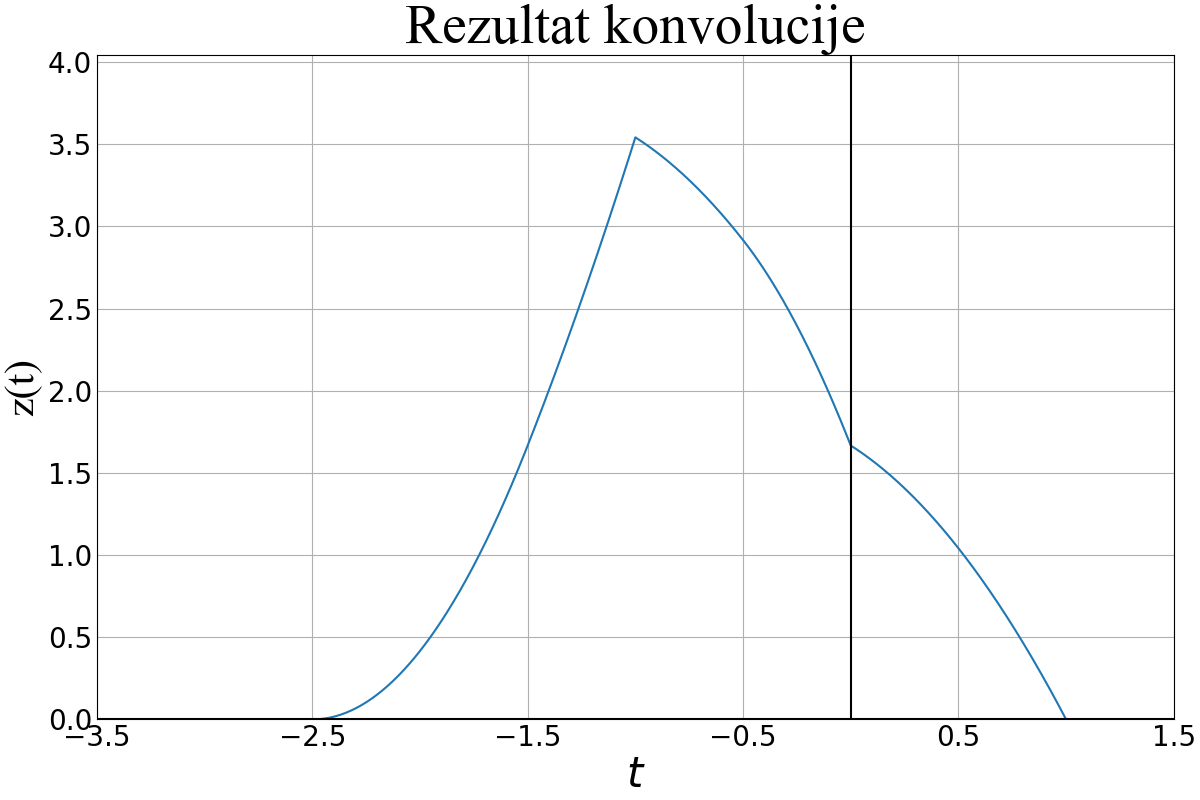
\includegraphics[width=\textwidth]{Images/zadatak2pic2.png}
		\caption{Signal $z(t) = x(t) *y(t)$}\label{fig:slika6}
	\end{figure*}\\
	\noindent{Za skiciranje grafika korišćen je sledeći kod u programskom jeziku Python:}
	\lstinputlisting[language=Python, caption={Kod za generisanje grafika sa Slike \ref{fig:slika6}.}]{Codes/zadatak2a2.py}
	
	\subsection[Drugi deo]{Analitički odrediti i skicirati konvoluciju signala $w[n]$ i $z[n]$}
	\vspace{-15pt}
	\begin{flalign}
		w[n] &= 0.5^n\big(u[n+2] - u[n-2]\big)\label{eq:wofn} \\
		z[n] &= 2u[n] \label{eq:zofn}
	\end{flalign}
	\indent Neka je rezultat konvolucije signala $w[n]$ i $z[n]$ signal $\gamma[n]$. Signal $\gamma[n]$ je sada definisan sa:
	\begin{equation}
		\gamma[n] = w[n] * z[n] = \sum_{k = -\infty}^{+\infty}z[k]\cdot w[n-k] \label{eq:discreteconvolution}
	\end{equation}
	\clearpage
	\indent Zamenom definicija jednačina \eqref{eq:wofn} i \eqref{eq:zofn} u definiciju \eqref{eq:discreteconvolution} možemo izračunati signal $\phi[n]$:
	\begin{flalign*}
		\gamma[n] &\quad= w[n] * z[n] = \sum_{k = -\infty}^{+\infty}z[k]\cdot w[n-k] \label{eq:discreteconvolution}\\
		&\quad= \sum_{k = -\infty}^{+\infty} 2u[k]\cdot w[n-k]\\
		&\quad= 2\sum_{k = 0}^{+\infty}w[n-k] = \left\{
		\begin{array}{l}
			m = n - k\\
			\quad
		\end{array}\right\}\\
		&\quad= 2\sum_{m =n}^{-\infty}w[m] = 2\sum_{m = -\infty}^{n} 0.5^m\big(u[m+2] - u[m-2]\big)\\\\
		\gamma[n] &\quad= \left\{
			\begin{array}{ll}
				0&,\quad n < -2 \\
				2\sum_{m = -2}^{n} 0.5^m&,\quad n \ge -2 \wedge n < 1 \\
				2\sum_{m = -2}^{1} 0.5^m&,\quad n \ge 1
			\end{array}\right.\\
		\gamma[n] &\quad= \left\{
			\begin{array}{ll}
				0&,\quad n < -2 \\
				2\sum_{m = 0}^{n+2} 0.5^{m-2}&,\quad n \ge -2 \wedge n < 1 \\
				2\sum_{m = 0}^{3} 0.5^{m-2}&,\quad n \ge 1
			\end{array}\right.\\
		\gamma[n] &\quad= \left\{
			\begin{array}{ll}
				0&,\quad n < -2 \\
				2\cdot4\sum_{m = 0}^{n} 0.5^{m}&,\quad n \ge -2 \wedge n < 1 \\
				2\cdot4\sum_{m = 0}^{3} 0.5^{m}&,\quad n \ge 1
			\end{array}\right.\\
		\gamma[n] &\quad= \left\{
			\begin{array}{ll}
				0&,\quad n < -2 \\
				8\cdot\frac{1 - 0.5^{n+3}}{1 - 0.5}&,\quad n \ge -2 \wedge n < 1 \\
				8\cdot\frac{1 - 0.5^4}{1 - 0.5}&,\quad n \ge 1
			\end{array}\right.\\
	\end{flalign*}
	\noindent Za konačan analitički oblik konvolucije signala dobijamo: 
	\begin{equation}
		\gamma[n] = \left\{
		\begin{array}{ll}
			0&,\quad n < -2 \\
			16\big(1 - 0.5^{n+3}\big)&,\quad n \ge -2 \wedge n < 1 \\
			15&,\quad n \ge 1
		\end{array}\right.
	\end{equation}
	\clearpage
	\noindent Na sledećoj slici prikazan je grafik rezultata konvolucije
	\begin{figure*}[ht]
		\centering
		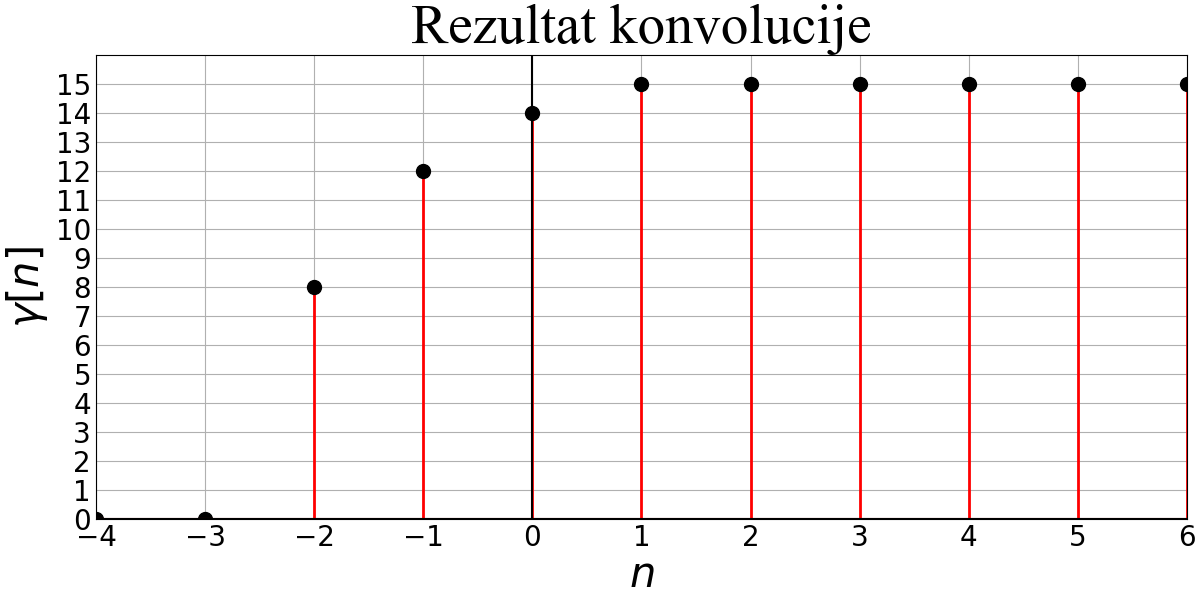
\includegraphics[width=\textwidth]{Images/zadatak2pic3.png}
		\caption{Signal $\gamma[n] = w[n] * w[n]$}\label{fig:slika7}
	\end{figure*}
	\FloatBarrier
	\noindent{Za skiciranje grafika korišćen je sledeći kod u programskom jeziku Python:}
	\lstinputlisting[language=Python, caption={Kod za generisanje grafika sa Slike \ref{fig:slika7}.}]{Codes/zadatak2b.py}
	\clearpage
	
	\section{Zadatak 3.}
	\Large{Osnovne osobine signala}
	\normalsize{}
	
	\subsection[Prvi deo]{Analitičkim postupkom odrediti da li je sistem S:}
	\begin{itemize}[noitemsep, partopsep=0pt,itemindent=20pt]
		\item linearan
		\item stacionaran
		\item sa memorijom
		\item kauzalan
		\item stabilan
	\end{itemize}
	\indent \large{Sistem S je definisan sa: $y(t) = x(2t)\cdot u(t)$}\\
	
	\noindent\textbf{Linearnost}\\
	\noindent Definišemo sledeće signale:
	\begin{flalign*}
		&y_1(t) = x_1(2t)u(t) &&y_2(t) = x_2(2t)u(t) &&x_3(t) = ax_1(t) + bx_2(t)
	\end{flalign*}
	Dalje imamo
	\begin{flalign*}
		y_3(t) = x_3(t)u(t) &\quad\Rightarrow y_3(t) = \big(ax_1(2t) + bx_2(2t)\big)u(t) \\
		&\quad\Rightarrow y_3(t) = ax_1(2t)u(t) + bx_2(2t)u(t)\\
		&\quad\Rightarrow y_3(t) = ay_1(t) + by_2(t)
	\end{flalign*}
	Vidimo da je \underline{sistem linearan}.\\
	\noindent\textbf{\\Stacionarnost}
	\begin{flalign*}
		&y(t-t_0) = x(2(t-t_0))\cdot u(t-t_0) = x(2t-2t_0)u(t-t_0)\\
		&x_p(t) = x(t-t_0)\\
		&y_p(t) = x_p(2t)\cdot u(t) = x(2t - t_0) \cdot u(t) \ne y(t-t_0)
	\end{flalign*}
	Vidimo da \underline{sistem nije stacionaran}.\\
	\clearpage
	\noindent\textbf{\\Memorija}\\
	Signal $y(t)$ ne zavisi od prethodnih vrednosti drugih signala, ali zavisi od budućih vrednosti signala $x_t$, tako da sistem \underline{ima memoriju}.\\
	\noindent\textbf{\\Kauzalnost}\\
	Signal $y(t)$ u trenutku $t$ zavisi od signala $x$ u trenutku $2t$, tako da sistem \underline{nije kauzalan}.\\
	\noindent\textbf{\\Stabilnost} 
	\begin{center}
		$(\exists B_1)(\forall t) |x(t)| < B1 \Rightarrow (\exists B_2)(\forall t) |y(t)| < B_2$
	\end{center}
	Neka postoji $B_1$, takvo da $|x(t)| < B_1$ za svako $t$.
	\begin{flalign*}
		|x(t)| \le B_1 &\Rightarrow |y(t)| = |x(2t)\cdot u(t)| = |x(t)|\cdot |u(t)| \\
		&\Rightarrow |y(t)| \le B_1|u(t)| \le B_1 = B_2
	\end{flalign*}
	Odavde vidimo da je \underline{sistem BIBO stabilan}.
	\clearpage
	
	\subsection[Drugi deo]{Analitičkim postupkom utvrditi da li je sistem L:}
	\begin{itemize}[noitemsep, partopsep=0pt,itemindent=20pt]
		\item linearan
		\item stacionaran
		\item sa memorijom
		\item kauzalan
		\item stabilan
	\end{itemize}
	\indent \large{Sistem L je definisan sa: $y[n] = \sum_{k = n-2}^{n} \big(2x[k+1]\big)$}\vspace{5pt}\\
	Prvo sređujemo izraz za $y[n]$ kako bi lakše odredili osobine sistema
	\begin{flalign*}
		y[n] &= \sum_{k = n-2}^{n} \big(2x[k+1]\big) = \left\{
			\begin{array}{l}
				m = k + 1 \\
				\quad
			\end{array}\right\}\\
		y[n] &= \sum_{k = n-1}^{n+1}2x[k]
	\end{flalign*}

	\noindent\textbf{Linearnost}\\
	\noindent Definišemo sledeće signale:
	\begin{flalign*}
		&y_1[n] = \sum_{k = n-1}^{n+1} \big(2x_1[k]\big) &&y_2[n] = \sum_{k = n-1}^{n+1} \big(2x_2[k]\big) &&x_3[n] = ax_1[n] + bx_2[n]
	\end{flalign*}
	Dalje imamo
	\begin{flalign*}
		y_3[n] = \sum_{k = n-1}^{n+1} \big(2x_3[k]\big) &\quad\Rightarrow y_3[n] = \sum_{k = n-1}^{n+1}2\big(ax_1[k] + bx_2[k]\big) \\
		&\quad\Rightarrow y_3[n] = \sum_{k = n-1}^{n+1}\Big(a\big(2x_1[k]\big) + b\big(2x_2[k]\big)\Big)\\
		&\quad\Rightarrow y_3[n] = a\sum_{k = n-1}^{n+1}2x_1[k] + b\sum_{k = n-1}^{n+1}2x_2[k]\\
		&\quad\Rightarrow y_3[n] = ay_1[n] + by_b[n]
	\end{flalign*}
	Vidimo da je \underline{sistem linearan}.\\
	\noindent\textbf{\\Stacionarnost}
	\begin{flalign*}
		&y[n-n_0] = \sum_{k = n-n_0-1}^{n-n_0+1}2x[k]\\
		&x_p[n] = x[n-n_0]\\
		&y_p[n] = \sum_{k = n-1}^{n+1}2x_p[k] = \sum_{k = n-1}^{n+1}2x[k-n_0] = \left\{
		\begin{array}{l}
			k - n_0 = m \\
			\quad
		\end{array}\right\}\\
		&y_p[n] = \sum_{k = n-n_0-1}^{n-n_0+1}2x[k] = y[n-n_0]
	\end{flalign*}
	Vidimo da je \underline{sistem stacionaran}.\\
	\noindent\textbf{\\Memorija}
	\begin{flalign*}
		y[n] = 2\cdot\big( x[n-1] + x[n] + x[n+1] \big)
	\end{flalign*}
	Vrednost signala $y[n]$ u trenutku $n$ zavisi od vrednosti ulaznog signala u trenutku $n-1$, tako da sistem \underline{ima memoriju}.\\
	\noindent\textbf{\\Kauzalnost}\\
	Vrednost signala $y[n]$ u trenutku $n$ zavisi od vrednosti ulaznog signala u trenutku $n + 1$, pa sistem \underline{nije kauzalan}.\\
	\noindent\textbf{\\Stabilnost} 
	\begin{center}
		$(\exists B_1)(\forall n) |x[n]| < B1 \Rightarrow (\exists B_2)(\forall n) |y[n]| < B_2$
	\end{center}
	Neka postoji $B_1$, takvo da $|x[n]| < B_1$ za svako $n$.
	\begin{flalign*}
		|x[n]| \le B_1 &\Rightarrow |y[n]| = \Big|\sum_{n-1}^{n+1}2x[k]\Big| \le 2\sum_{n-1}^{n+1}\Big|x[k]\Big|\\
		&\Rightarrow |y[n]| \le 6B_1 = B_2
	\end{flalign*}
	Odavde vidimo da je \underline{sistem BIBO stabilan}.
	\clearpage
	

	\section{Zadatak 4.}
	\Large{Furiheovi redovi}
	\normalsize{}
	
	\subsection[Prvi deo]{Napisati analitički oblik signala $v(t)$, odrediti njegovu osnovnu periodu T i učestanost $\omega_0$, i izvesti izraz za koeficijente Furijeovog reda $a_k$}
	\begin{figure*}[ht]
		\centering
		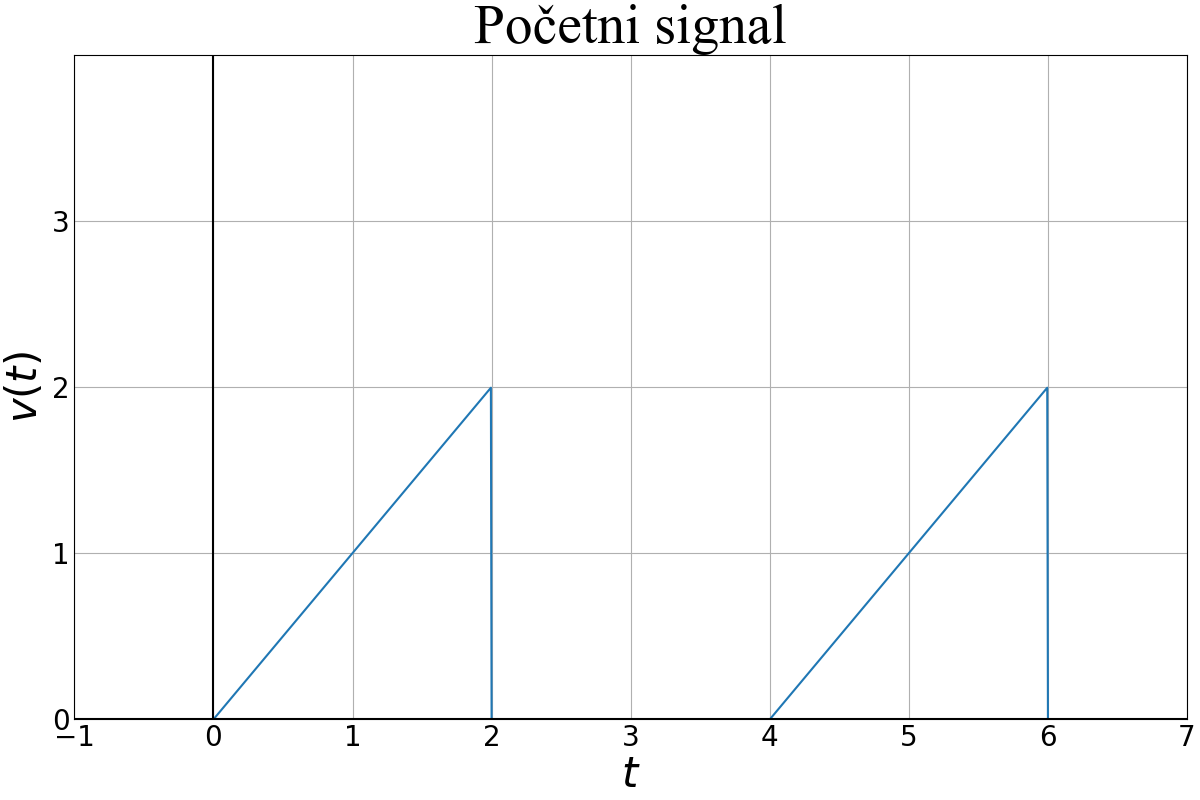
\includegraphics[width=\textwidth]{Images/zadatak4pic1.png}
		\caption{Signal $v(t)$}\label{fig:slika8}
	\end{figure*}
	\noindent Sa slike se vidi da je period signala $T = 4s$. Odavde sledi da je kružna učestanost $\omega_0 = \frac{2\pi}{T} = \frac{\pi}{2} rad/s$. Sa slike se može očitati i analitčki oblik signala $v(t)$:
	\begin{equation}
		v(t) = \sum_{k=-\infty}^{\infty}\big(t-4k\big)\big( u(t-4k) - u(t - 4k-2)\big)
	\end{equation}
	\clearpage
	\noindent{Za skiciranje grafika korišćen je sledeći kod u programskom jeziku Python:}
	\lstinputlisting[language=Python, caption={Kod za generisanje grafika sa Slike \ref{fig:slika8}}]{Codes/zadatak4a1.py}
	\clearpage
	
	\noindent \textbf{Izvođenje koeficijenata Furijeovog reda\\}
	Furijeov red funkcije $v(t)$ dat je sumom:
	\begin{equation}
		v(t) = \sum_{k=-\infty}^{+\infty}a_k\cdot e^{j\omega_0kt}
	\end{equation}
	gde su koeficijenti $a_k$ definisani sa:
	\begin{equation}
		a_k = \frac{1}{T}\int\limits_{T}v(t)e^{-j\omega_0kt}dt\label{eq:fouriercoeff}
	\end{equation}
	Odredimo sada koeficijente Furijeovog reda:
	\begin{flalign}
		a_k &\quad= \frac{1}{T}\int\limits_{T}v(t)e^{-j\omega_0kt}dt = \frac{1}{4}\int_0^2 te^{-j\omega_0kt}dt = \left\{
			\begin{array}{lll}
				u=t&, &dv=e^{-j\omega_0kt}\\
				du=dt&, &v=-\frac{1}{k\omega_0k}e^{-j\omega_0kt}
			\end{array}
		\right\}\notag\\
		a_k &\quad= \frac{1}{4} \Bigg(
			-\frac{1}{j\omega_0k}te^{-j\omega_0kt}\Big|_0^2
			+\frac{1}{j\omega_0k}\int_0^2 e^{-j\omega_0kt}dt
		\Bigg)\notag\\
		a_k &\quad= \frac{1}{4} \Bigg(
			-\frac{1}{j\omega_0k}\cdot 2e^{-jk\pi}
			+\frac{1}{j\omega_0k}\cdot \Big(-\frac{1}{j\omega_0k}\Big)
			e^{-j\omega_0kt}\Bigg|_0^2
		\Bigg)\notag\\
		a_k &\quad= \frac{1}{4}\Bigg(
			-\frac{2}{j\frac{\pi}{2}k}\cdot e^{-jk\pi}
			+ \frac{1}{\big(\frac{\pi}{2}\big)^2 k^2}
			\Big(
				e^{-jk\pi} - 1
			\Big)
		\Bigg)\notag\\
		a_k &\quad= \frac{1}{4}\Bigg(
			-\frac{4}{j\pi k}\cdot \big(e^{-j\pi}\big)^k
			+ \frac{4}{\pi^2 k^2}
			\Big(
				\big(e^{-j\pi}\big)^k - 1
			\Big)
		\Bigg)\notag\\
		a_k &\quad= \Bigg(
			\frac{j}{\pi k}\cdot (-1)^k
			- \frac{1}{\pi^2 k^2}
			\Big(1 - (-1)^k\Big)
		\Bigg)\label{eq:fouriercoefffinal}
	\end{flalign}
	\noindent Vidimo da koeficijent $a_k$ nije definisan relacijon \eqref{eq:fouriercoefffinal} za $k = 0$, tako da koeficijent $a_0$ moramo računati posebno, koristeći se relacijom \eqref{eq:fouriercoeff} i uzimajući $k = 0$.
	\begin{flalign}
		a_0 = \frac{1}{T}\int\limits_{T}v(t)dt = \frac{1}{4}\int_0^4 v(t)dt = \frac{1}{4}\int_0^2 tdt = \frac{1}{4} \cdot \frac{1}{2}t^2 \Big|_0^2 = \frac{1}{8}\cdot 4 = \frac{1}{2}
	\end{flalign}
	Konačno, koeficijenti $a_k$ Furijeovog reda funkcije $v(t)$ definisani su sa
	\begin{equation}
		a_k = \left\{
			\begin{array}{lll}
				&\frac{1}{2}&,\quad k = 0\\
				&j\frac{1}{4\pi}(-1)^k - \frac{1}{\pi^2k^2}\big(1 - (-1)^k\big)&,\quad k \ne 0
			\end{array}
		\right. \label{eq:fouriercoefffinal2}
	\end{equation}
	\clearpage
	
	\subsection[Drugi deo]{k-ti harmonik $v_k(t)$ signala $v(t)$ može se odrediti kao:}
	\vspace{-8pt}
	\noindent $v_k(t) = a_{-k}e^{-jk\omega_0t} + a_{k}e^{jk\omega_0}t = 2Re\big\{a_ke^{jk\omega_0t}\big\} = A_k\cos(k\omega_0t+\phi_k)$, $k\ge1$\vspace{2pt}\\
	\vspace{2pt}
	\large{\textbf{Odrediti amplitude $A_k$ i faze $\phi_k$ za prva dva harmonika\\ $(k=1,2)$, i skicirati na istom grafiku signale $v(t)$, $v_1(t)$ i $v_2(t)$}}\\\\
	\normalsize{}
	\noindent Koeficijente $A_k$ i $\phi_k$ ćemo najlakše nalaziti iz relacije:
	\begin{equation}
		v_k(t) = 2Re\big\{a_ke^{jk\omega_0t}\big\} = A_k\cos(k\omega_0t+\phi_k)\label{eq:coeffrelation}
	\end{equation}
	\noindent Odredimo prvo prvi harmonik $v_1(t)$.\\
	Prvo ćemo odrediti koeficijent $a_1$
	\begin{flalign}
		a_1 &= j\frac{1}{\pi}(-1)^1 - \frac{1}{\pi^2}\big(1-(-1)^1\big)\notag\\
		a_1 &= -j\frac{1}{pi} - \frac{1}{\pi^2}(1 + 1)\notag\\
		a_1 &= -\frac{2}{\pi^2} - j\frac{1}{pi}\label{eq:foureircoeffa1}
	\end{flalign}
	\indent Za nalaženje koeficijenata $A_1$ i $\phi_1$ najpogodnija je relacija $v_1(t) = 2Re\big\{a_1 e^{k\omega_0t}\big\}$, tako da je potrebno izraziti koeficijent $a_1$ u obliku $|a_1|e^{j\theta_k}$.
	\begin{flalign}
		|a_1|=\sqrt{\Big(\frac{2}{\pi^2}\Big)^2 + \Big(\frac{1}{\pi}\Big)^2} = \sqrt{\frac{4}{\pi^4}+\frac{1}{\pi^2}}= \frac{1}{\pi^2}\sqrt{4+\pi^2}\label{eq:coeffa1mag}\\7
		\notag\\
		\theta_1 = \arg(a_1) =  \arctan\Bigg(\frac{-\frac{1}{\pi}}{-\frac{2}{\pi^2}}\Bigg) - \pi = \arctan\frac{\pi}{2} - \pi \label{eq:coefftheta1}
	\end{flalign}
	Ubacivanjem \eqref{eq:coeffa1mag} i \eqref{eq:coefftheta1} u izraz \eqref{eq:coeffrelation} dobijamo:
	\begin{flalign}
		v_1(t) = 2Re\Bigg\{\frac{1}{\pi^2}\sqrt{4+\pi^2}e^{j\big(\arctan\frac{\pi}{2}-\pi\big)} e^{j\frac{\pi}{2}t}\Bigg\}\notag\\
		A_1\cos(k\frac{\pi}{2} + \phi_k) = \frac{2}{\pi^2}\sqrt{4+\pi^2} \cos\Big(\frac{\pi}{2}t + \arctan\frac{\pi}{2}-\pi\Big)\label{eq:firstharmoniccoeff}
	\end{flalign}
	Izjednačavanjem koeficijenata konačno imamo:\\
	\indent\begin{minipage}{0.5\textwidth}
		\begin{flalign}
			A_1 = \frac{2}{\pi^2}\sqrt{4+\pi^2}
		\end{flalign} 
	\end{minipage}%
	\begin{minipage}{0.5\textwidth}
		\begin{flalign}
			\phi_1 = \arctan\frac{\pi}{2}-\pi
		\end{flalign}
	\end{minipage}\vskip1em
	\clearpage
	Istim postupkom sada određujemo drugi harmonik $v_2(t).$
	Određujemo koeficijent $a_2$:
	\begin{equation}
		a_2= j\frac{1}{2\pi}(-1)^2 - \frac{1}{4\pi^2}\big(1-(-1)^2\big) = j\frac{1}{2\pi}
	\end{equation}
	Odredimo sada $|a_2|$ i $\theta_2$:\\
	\indent\begin{minipage}{0.5\textwidth}
		\begin{flalign}
			|a_2| = \Big|j\frac{1}{2\pi}\Big| = \frac{1}{2\pi}
		\end{flalign} 
	\end{minipage}%
	\begin{minipage}{0.5\textwidth}
		\begin{flalign}
			\theta_2 = \frac{\pi}{2}
		\end{flalign}
	\end{minipage}\vskip1em
	\noindent Izjednačavanjem koeficijenata, kao u \eqref{eq:firstharmoniccoeff}, dobijamo:\\
	\indent\begin{minipage}{0.5\textwidth}
		\begin{flalign}
			A_2 = \frac{1}{\pi}
		\end{flalign} 
	\end{minipage}%
	\begin{minipage}{0.5\textwidth}
		\begin{flalign}
			\phi_2 = \frac{\pi}{2}
		\end{flalign}
	\end{minipage}\vskip2em
	\noindent Zamenom dobijenih koeficijenata harmonika u definiciju $k$-tog harmonika dobija se:
	\begin{flalign}
		v_1(t) &= \frac{2}{\pi^2}\sqrt{4+\pi^2} \cos\Bigg(\frac{\pi}{2}t +	 \arctan\frac{\pi}{2}-\pi\Bigg)\\
		v_2(t) &= \frac{1}{\pi}\cos\Big(\pi t + \frac{\pi}{2}\Big)
	\end{flalign}
	\noindent Na sledećoj slici može se videti grafik sa signalima $v(t)$, $v_1(t)$ i $v_2(t)$:
	\begin{figure*}[ht]
		\centering
		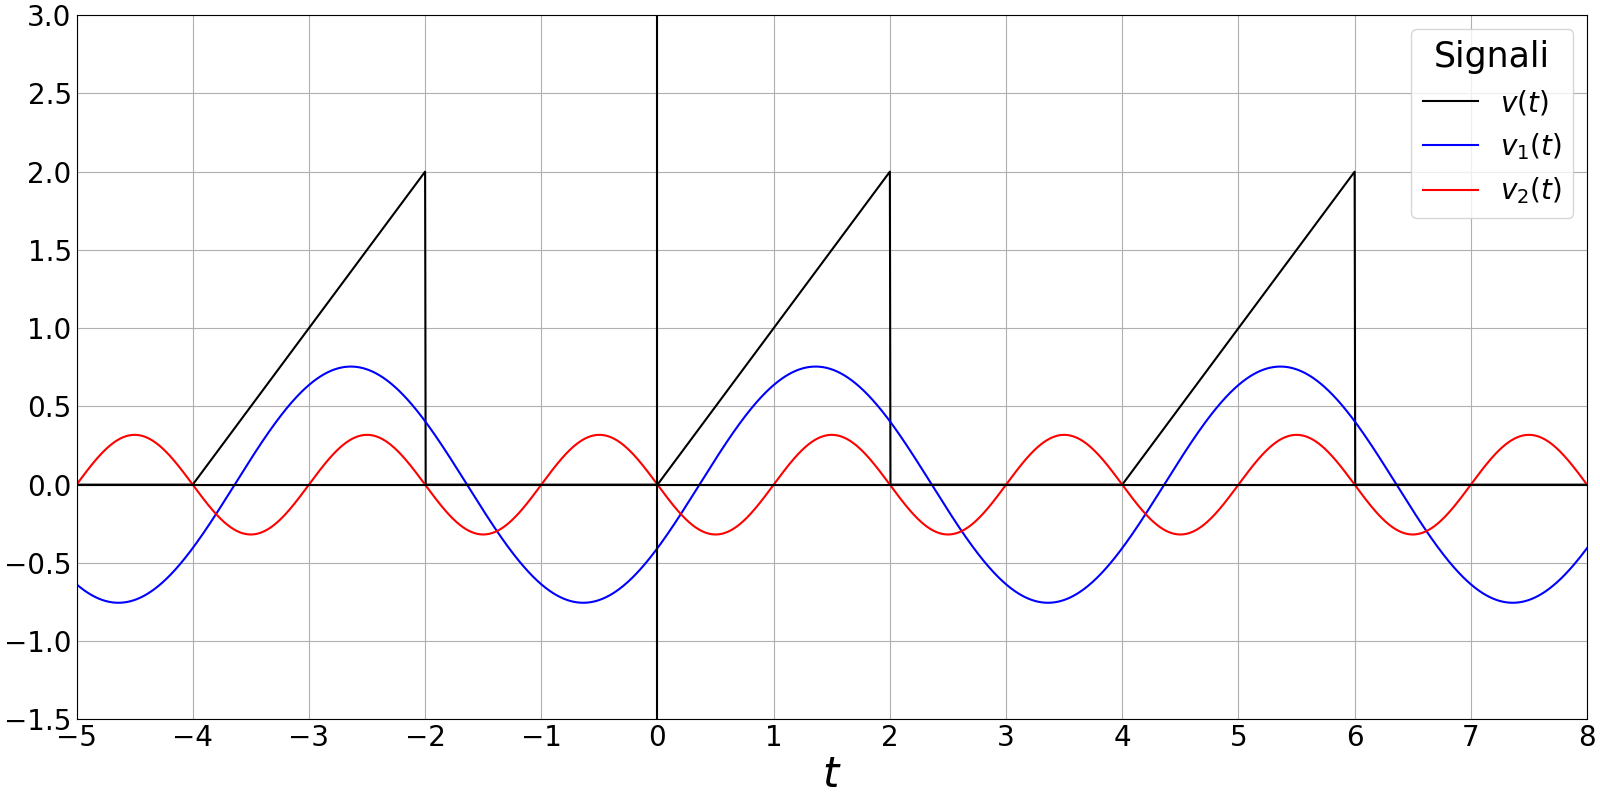
\includegraphics[width=\textwidth]{Images/zadatak4pic2.png}
		\caption{Signali $v(t)$, $v_1(t)$ i $v_2(t)$}\label{fig:slika9}
	\end{figure*}
	\FloatBarrier
	\pagebreak
	\noindent{Za skiciranje grafika korišćen je sledeći kod u programskom jeziku Python:}
	\lstinputlisting[language=Python, caption={Kod za generisanje grafika sa Slike \ref{fig:slika9}}]{Codes/zadatak4b.py}
	
	\pagebreak
	\subsection[Treći deo]{Skicirati na istom grafiku originalni signal $v(t)$ i aproksimaciju:}
	\vspace{-15pt}
	\large{\begin{equation}
		\hat{v}_1(t) = \sum_{k=-1}^{1} a_k e^{jk\omega_0t}= a_0 + v_1(t)\notag
	\end{equation}}
	\normalsize{}
	Zamenom izračunatih vrednosti koeficijenata dobijamo da je:
	\begin{equation}
		\hat{v}_1(t) = \frac{1}{2} + \frac{2}{\pi^2}\sqrt{4+\pi^2}\cdot\cos\Big(\frac{\pi}{2}t+\arctan\frac{\pi}{2} - \pi\Big)
	\end{equation}
	\noindent Na sledećoj slici može se videti grafik sa signalima $v(t)$i $\hat{v}_1(t)$:
	\begin{figure*}[ht]
		\centering
		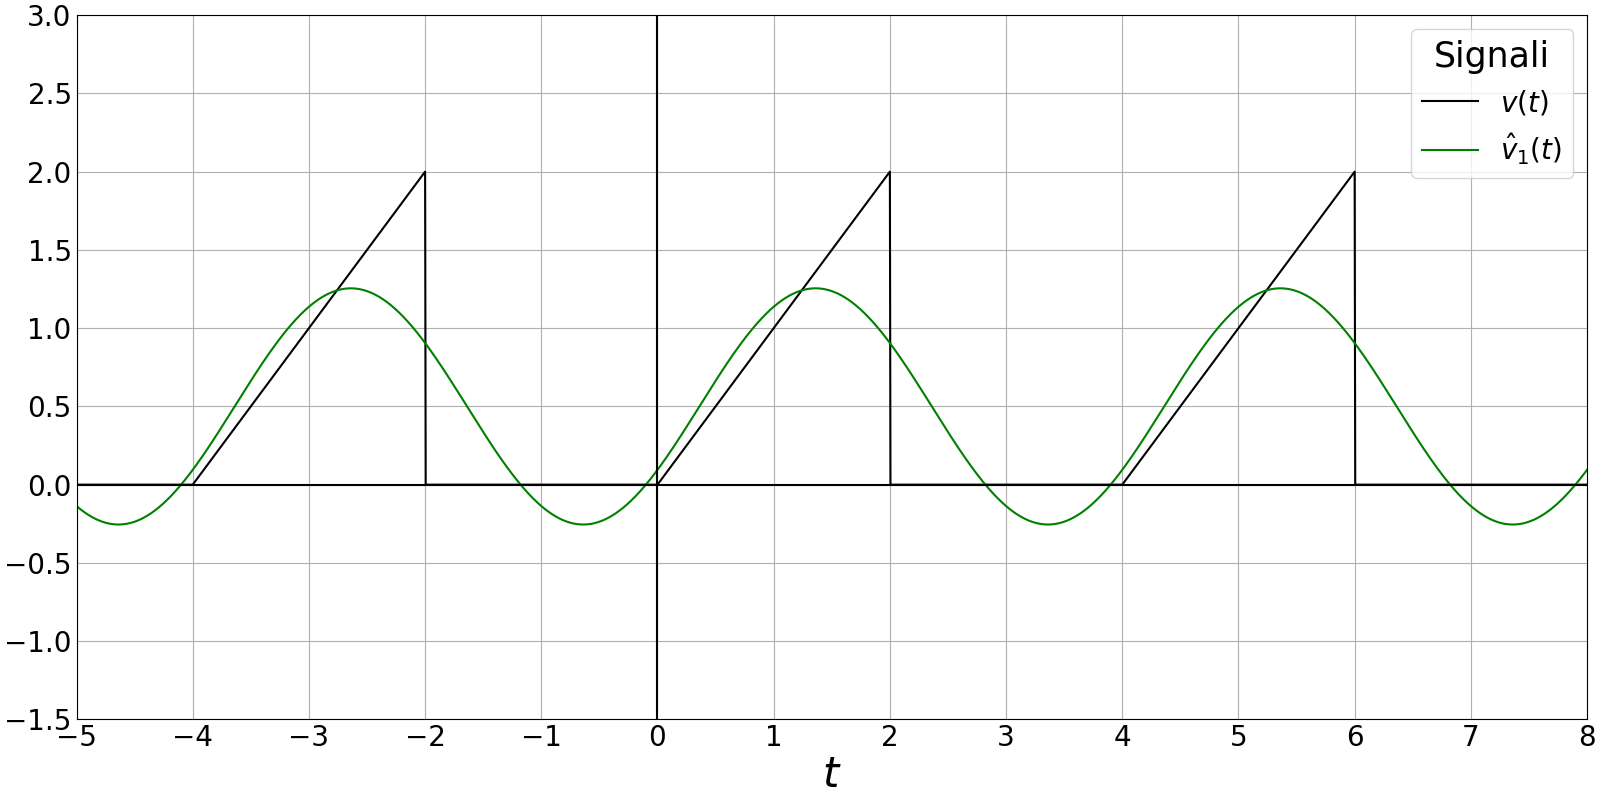
\includegraphics[width=\textwidth]{Images/zadatak4pic3.png}
		\caption{Signali $v(t)$i $\hat{v}_1(t)$}\label{fig:slika10}
	\end{figure*}
	\FloatBarrier
	\pagebreak
	\noindent{Za skiciranje grafika korišćen je sledeći kod u programskom jeziku Python:}
	\lstinputlisting[language=Python, caption={Kod za generisanje grafika sa Slike \ref{fig:slika10}}]{Codes/zadatak4c.py}
	
	\subsection[Četvrti deo]{Grafički prikazati zavisnost modula koeficijenta od indeksa $k$, za $0\le k \le 3$}
	
	Koeficijenti Furijeovog reda $a_k$ signala $v(t)$ dati sa \eqref{eq:fouriercoefffinal2} mogu se napisati i u obliku:
	\begin{equation}
		a_k = \left\{
		\begin{array}{lll}
			\frac{1}{2}&,\quad k = 0\\
			\frac{j}{k\pi}&,\quad k = 2p \\
			-\frac{2}{\pi^2k^2}-j\frac{1}{k\pi}&,\quad k = 2p + 1
		\end{array}
		\right. 
	\end{equation}
	Odavde lako možemo naći moduo koeficijenta $a_k$:
	\begin{equation}
		|a_k| = \left\{
		\begin{array}{lll}
			\frac{1}{2}&,\quad k = 0\\
			\frac{1}{k\pi}&,\quad k = 2p \\
			\frac{1}{k^2\pi^2}\sqrt{4+k^2\pi^2}&,\quad k = 2p + 1
		\end{array}
		\right. \label{eq:fouriercoeffmodule}
	\end{equation}
	Kako je $a_k = a_{-k}^* \Rightarrow |a_k| = |a_{-k}|$ pomoću \eqref{eq:fouriercoeffmodule} možemo lako izračunati module koeficijenata za $|k|\le 3$
	\begin{flalign}
		|a_1| &=|a_{-1}|=\frac{1}{\pi^2}\sqrt{4+\pi^2} \approx 0.377\\
		|a_2| &= |a_{-2}| = \frac{1}{2\pi} \approx 0.159\\
		|a_3| &= |a_{-3}| = \frac{1}{9\pi^2}\sqrt{4+9\pi^2} 	\approx 0.109
	\end{flalign}
	\clearpage
	\noindent Na sledećoj slici može se videti grafik sa modulima koeficijenata $a_k$ za $|k|\le 3$:
	\begin{figure*}[ht]
		\centering
		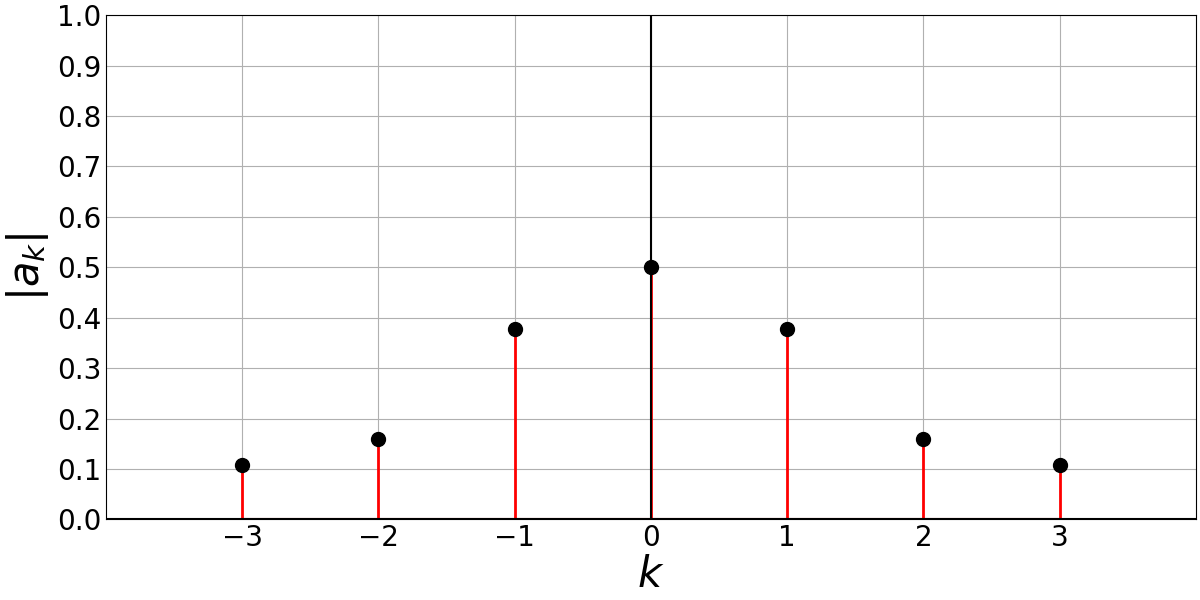
\includegraphics[width=\textwidth]{Images/zadatak4pic4.png}
		\caption{Moduli koeficijenata $a_k$}\label{fig:slika11}
	\end{figure*}
	\FloatBarrier
	\noindent{Za skiciranje grafika korišćen je sledeći kod u programskom jeziku Python:}
	\lstinputlisting[language=Python, caption={Kod za generisanje grafika sa Slike \ref{fig:slika11}}]{Codes/zadatak4d.py}
	
	\subsection[Peti deo]{Ispitati konvergentnost Furijeovog reda  signala u srednje-kvadratnom smislu}
	
	Furijeov red signala $v(t)$ je konvergentan u srednje-kvadratnom smislu ako je integral
	\begin{equation}
		\int\limits_T \big|v(t)\big|^2 dt
	\end{equation}
	konačnan, tj. konvergentan. Računajući integral
	\begin{flalign*}
		I = \int\limits_T \big|v(t)\big|^2 dt = \int_0^4 \big|v(t)\big|^2 dt = \int_0^2|t|^2dt = \frac{t^3}{3} \Big|_0^2 = \frac{8}{3} < +\infty
	\end{flalign*}
	vidimo da on konvergira. Možemo zaključiti da
	{\ulined Furijeov red konvergira u srednje-kvadratnom smislu}.
	\clearpage
	\lstlistoflistings
\end{document}
